\chapter{Ergebnisse}
Jedes Messverfahren muss sich vor allem durch seine Genauigkeit behaupten. Im folgenden Kapitel werden in dieser Hinsicht die Ergebnisse vorgestellt, die das in Kapitel \ref{chap:Implementierung} implementierte Verfahren erbracht hat. Dabei wird auch darauf eingegangen, warum die erläuterten Ansätze verfolgt wurden, welche Schwierigkeiten sich ergeben und inwiefern diese sich auf die Messergebnisse ausgewirkt haben. Für die folgenden Erklärungen wurde die ebenfalls vorliegende exemplarische Messreihe einer im Raum liegenden schiefen Ebene verwendet, welche sich aufgrund ihrer geometrisch einfachen Form leicht beschreiben und als Validierungsobjekt verwenden lässt.   

\section{Laserlinienbestimmung}
\label{subsec:segmentierung}

Die Lokalisierung der Laserlinie bestimmt in Bildkoordinaten, welche Teile des Bildes für die Messung interessant sind. Jegliche Ungenauigkeiten, die in diesem Schritt auftreten, propagieren sich also unweigerlich in den Folgeschritten zu immer größeren Messfehlern. Eine sorgfältige Bildverarbeitung ist hier also von hoher Bedeutung.\bigbreak
Wie in Abschnitt \ref{subsec:Farbkalibrierung} und \ref{subsec:LaserLinieBestimmung} beschrieben, wird für die Segmentierung der Laserlinie auf einen globalen Farbgrenzwert gesetzt. Dieser Ansatz erweist zwar eine geringe Komplexität, ist aber nicht ohne Nachteile. In Abb. \ref{fig:farbwerte} sind exemplarisch die Farbkanalwerte für die Pixel einer einzelnen Bildspalte aus einem ausgewählten Bild (welches in Abb. \ref{fig:LaserLinieExtraktion} ganz oben zu sehen ist) sowohl im RGB- als auch im YCbCr-Farbraum dargestellt. Dabei befinden sich auf der X-Achse die Reihenindizes und auf der Y-Achse die Kanalwerte im Bereich von \(0\) bis \(255\). Wie man der Abbildung erkennen kann, befindet sich die Laserlinie im X-Achsenabschnitt zwischen ca. \(370\) bis \(380\), erkennbar durch den hohen Ausschlag im Rot-Kanal. Möchte man nun einen globalen Farbgrenzwert ansetzen um die Laserlinie in ihrer gesamten Breite von ca. \(10\) Pixel zu erfassen und dabei alle anderen Bildanteile auszublenden, müssten alle Pixel mit einem Rotkanalwert von ca. unter \(50\) ausgeblendet (also geschwärzt) werden. Dabei bleiben aber noch die Pixel übrig, die sowohl einen hohen Rot- als auch einen hohen Blau und Grün-Anteil aufweisen und somit ebenfalls nicht zur Laserlinie gehören. Es würde sich nun also anbieten, für den Grün- und Blau-Kanal einen Obergrenzwert festzulegen, der zusätzlich alle Pixel schwärzt, deren Grün- und Blau-Anteile über diesen Grenzwerten liegen. Wie aus Abb. \ref{fig:farbwerte} allerdings hervorgeht, ist es nicht möglich, solche Grenzwerte zu finden und gleichzeitig alle Pixel der Laserlinie zu erhalten. Vor allem im X-Achsenabschnitt von \(0\) bis \(150\) sind die Grünkanalwerte nicht hoch genug um durch die Obergrenze geschwärzt zu werden und gleichzeitig die Pixel im X-Achsenabschnitt von \(370\) bis \(380\) intakt zu lassen (ähnliches gilt für die Blau-Werte in anderen Teilen des Bildes). Eine Alternative bestünde darin, den Rotkanal-Untergrenzwert zu erhöhen, um die hohen Rotkanalwerte im X-Achsenabschnitt von \(0\) bis \(150\) auszublenden, was allerdings in einer generellen Schmälerung der Laserliniensegmentierung resultiert.\linebreak
In der vorliegenden Implementierung wurde nun anstatt eines RGB- ein YCbCr-Grenzwert verwendet. Dieser ist ebenfalls in Abb. \ref{fig:farbwerte} abgebildet. Das geschilderte Problem lässt sich zwar auch in diesem Farbraum nicht gänzlich vermeiden, jedoch besser kontrollieren. Wie in der Abbildung zu sehen ist, kann mit einem Untergrenzwert von ca. \(150\) die Laserlinie in einem Großteil ihrer Breite erfasst werden ohne dabei andere Farbkanäle in Betracht ziehen zu müssen. Indem nur ein Grenzwert angepasst werden muss, eignet sich dieser Farbraum somit auch zur besseren automatischen Grenzwertfindung, welche sicherstellen soll, dass die Schmälerung der Laserliniensegmentierung minimal ausfällt.   
\bigbreak
Ohne eine lokale Betrachtung der Bilddaten lässt sich mit einem globalen Ansatz die Segmentierung der Laserlinie also nicht zur  Gänze beseitigen. Daher wird in der vorliegenden Implementierung wie in \ref{subsec:LaserLinieBestimmung} beschrieben darauf gesetzt, nach einer groben Lokalisierung auf Basis dieser ersten Segmentierung eine feinere Bestimmung auf Basis der umliegenden unsegmentierten Pixeldaten vorzunehmen. So wird der Nachteil eines globalen Farbgrenzwertes abgeschwächt ohne zu viel Komplexität hinzuzufügen. Die Ergebnisse der Laserlinienbestimmung bewegen sich dank dieses Ansatzes in einem akzeptablen Fehlerraum. In \ref{fig:LaserLinieExtraktion} ist eine mit dem Verfahren erkannte Laserlinie zu sehen, welche neben einem vom Benutzer vorgenommenen Goldstandard und vor dem Hintergrund des betreffenden Bildes dargestellt ist. Der Cr-Grenzwert der in diesem Beispiel gewählt wurde ist durch dass Verfahren ermittelt worden, welches in \ref{subsec:Farbkalibrierung} beschrieben wurde. Die Distanz zwischen der optimalen und der ermittelten Linie beträgt \(5.0443\) Pixel.

\begin{figure}
\centering 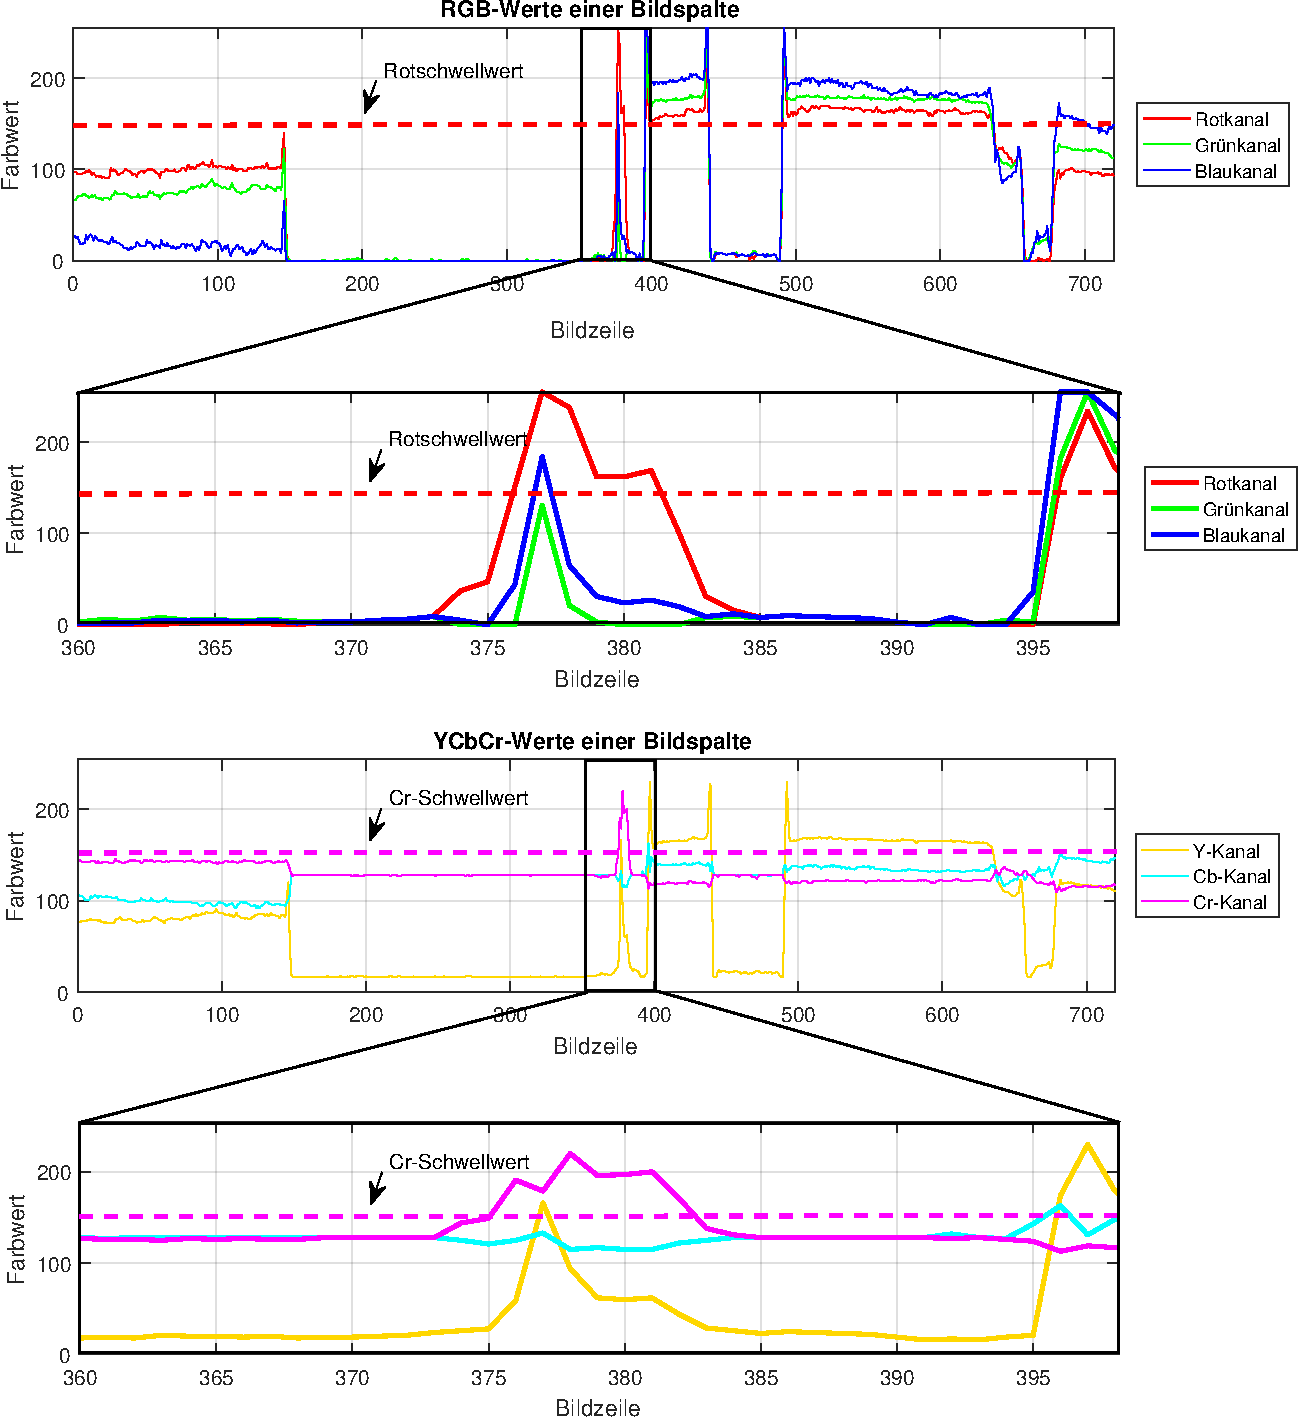
\includegraphics[width=\textwidth]{images/ColorAugmented4.pdf}
\caption[Farbkanäle einer einzelnen Bildspalte]{Farbkanäle der 701. Bildspalte des oberen Bildes aus Abb. \ref{fig:LaserLinieExtraktion}. Die vergrößerten Ausschnitte zeigen den Abschnitt genauer, auf dem sich die Laserlinie (die Bildzeilen von ca. 373 bis 383) befindet. Es ist zu erkennen, dass sich mit einem Minimalschwellwert im Rotkanal nicht alle Pixel außerhalb der Laserlinie aussortieren lassen: In den Bildzeilen von 500 bis ca. 650 sind zum Beispiel ebenfalls hohe Rotanteile. Die auf diese Weise nicht erfassten Pixel mit einem Maximalschwellwert im Blaukanal auszusortieren würde wiederum auch die Pixel im Laserlinien-Bereich aussortieren. Ähliche Probleme ergeben sich im Grünkanal. Im Vergleich dazu lässt sich im Cr-Kanal ein treffender Minimalschwellwert im Cr-Kanal ansetzen, mit dem die Laserlinie in annähernd voller Breite segmentiert wird und dabei alle anderen Pixel in der Bildspalte ausschwärzt.}\label{fig:farbwerte}
\end{figure}

\section{Messgenauigkeit}
Die Genauigkeit der Berechnung der Weltkoordinaten bestimmt wie erfolgreich das Messverfahren in seiner Gesamtheit funktioniert, da diese das angestrebte Endprodukt der Messung darstellen. Um diese Genauigkeit zu bestimmen, wurde für die vorliegende Implementierung die zu Eingang des Kapitels erwähnte schiefe Fläche zweimal vermessen: Einmal händisch um nötige Daten für die mathematische Beschreibung der Schräge zu sammeln, und einmal mit dem Lichtschnittverfahren um diese Messung mit der händischen Messung zu vergleichen. Durch die händische Messung lässt sich die Schräge mathematisch vergleichsweise einfach als eine durch vier Seiten begrenzte Ebene beschreiben und eignet sich daher zur Berechnung einer Metrik, mit der die Exaktheit des Verfahrens bewertet werden kann. Dafür wird für jede Weltkoordinate der kürzeste Abstand zur Ebene berechnet. Es wird immer der kürzeste Abstand zum jeweils nächsten Merkmal der Schräge ermittelt, also entweder zur Ebene an sich, zu einer der vier Seiten oder einer der vier Eckpunkte der Fläche. Anschließend wird das arithmetische Mittel dieser Abstände gebildet, um zu ermitteln, wie weit eine Koordinate im Durchschnitt von der eigentlichen Fläche entfernt ist. \linebreak
In \ref{fig:MessungSlope} ist die gemessene Punktewolke der Schräge entgegengestellt. Gemessen wurden hier \(2168\) Punkte, welche im Durchschnitt \(0.9083\) Millimeter mit einer Standardabweichung \(\sigma = 0.5360\) von  der optimalen Schräge entfernt liegen. \bigbreak

\begin{figure}
\centering 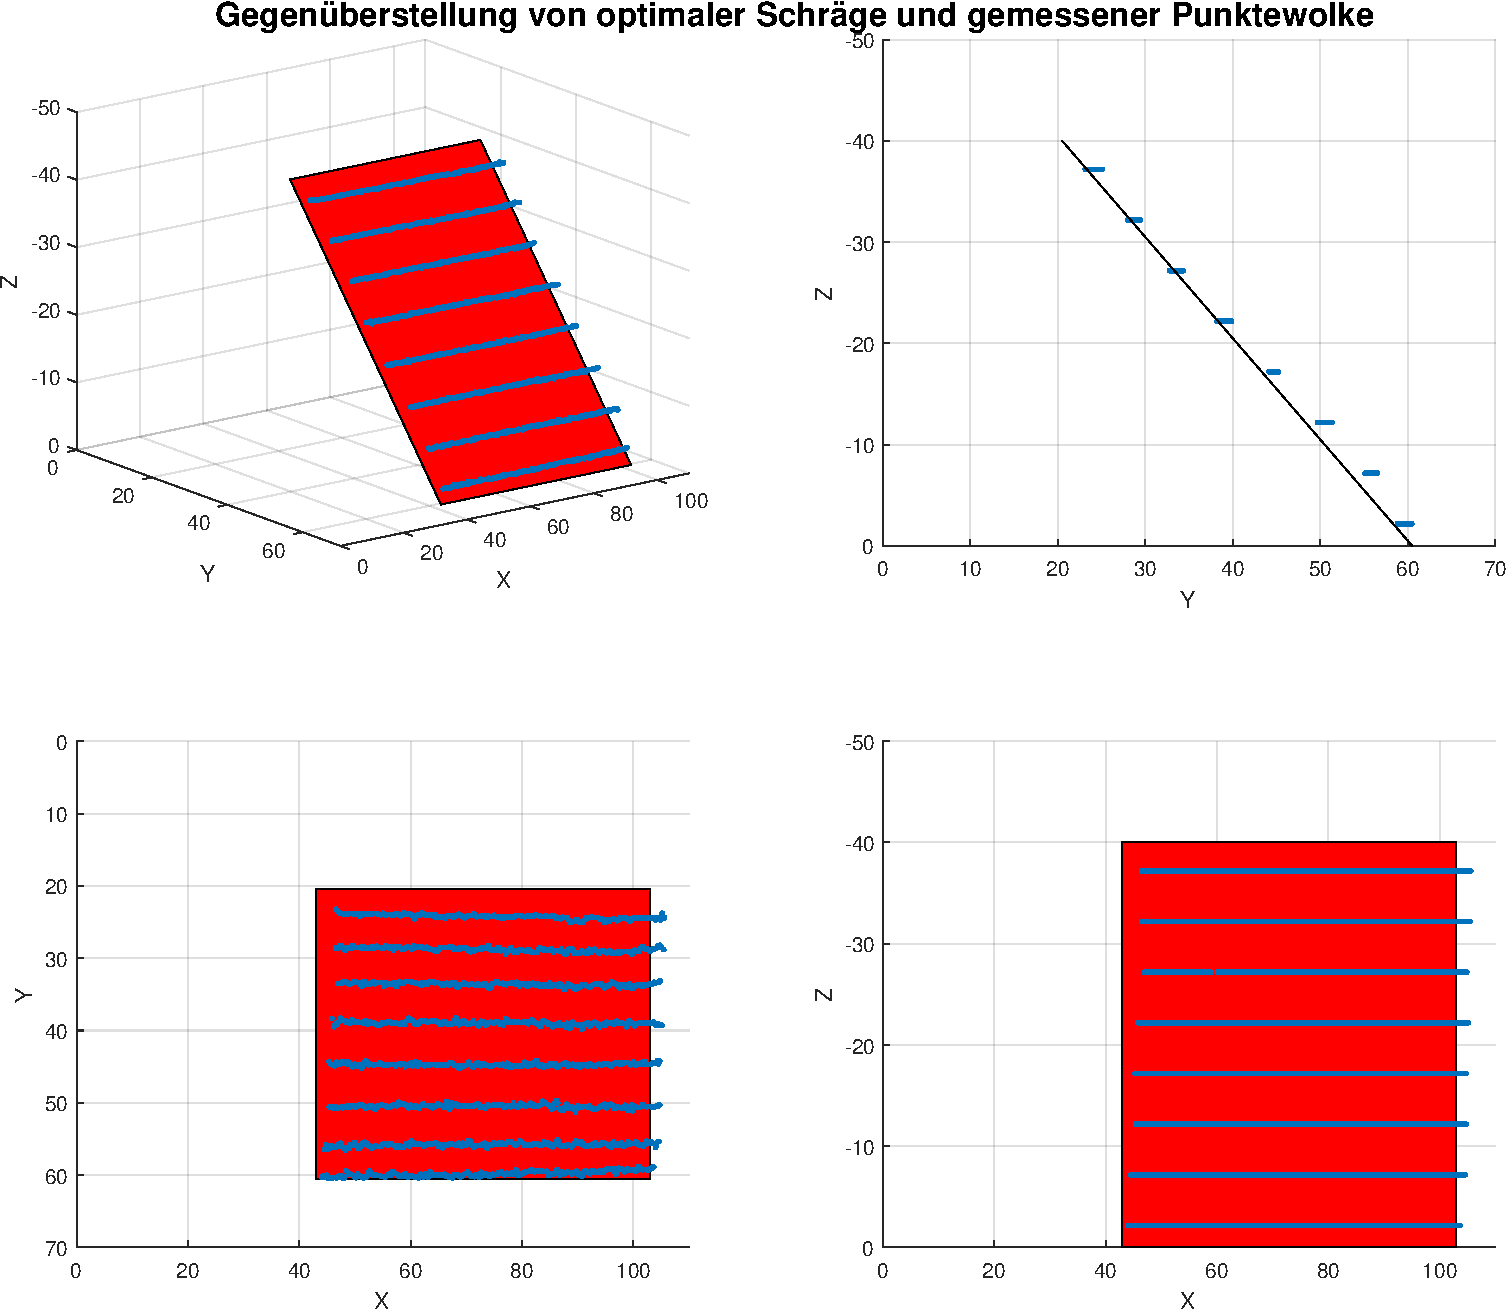
\includegraphics[width=\textwidth]{images/MessungBig.pdf}
\caption[Gegenüberstellung von optimaler Schräge und gemessener Punktewolke]{Gegenüberstellung von optimaler Schräge und gemessener Punktewolke}\label{fig:MessungSlope}
\end{figure}

Es ist auf der X-Y-Ebene zu sehen, dass die einzelnen vermessenen Punkte-Linien eine Schiefe aufweisen und nicht im perfekten rechten Winkel zur X-Achse stehen. Dies ist der Tatsache geschuldet, dass der Laser in der Bildaufnahmen nicht perfekt parallel zur Bodenebene steht. Als Resultat neigt sich auch auf den Bildern die Laserlinie mit einer minimalen Steigung, was den oben zu sehenden Effekt hervorbringt. Dies lässt sich vor allem mit erhöhter Sorgfalt während des Vermessens mildern, zeigt jedoch, dass Außeneinflüsse im direkten Vergleich zu mathematisch optimalen Konstrukten selten zur Gänze zu vermeiden sind.\linebreak
Ein Problem des Verfahrens liegt ebenfalls in der Gefahr, dass die mathematische Beschreibung des Validierungsobjektes das Objekt idealer beschreibt als in der Realität abgebildet. Somit kann die Messung zu einem gewissen Grad niemals an die mathematische Beschreibung heran reichen und der Messung wird auf diese Weise "`Unrecht getan"; sie wird also schlechter eingeschätzt als sie eigentlich ist. Dennoch kann bei genügender Sorgfalt der händischen Vermessung des Objektes damit gerechnet werden, dass die Metrik aussagekräftig ist. Auch wenn die verwendete Metrik nur für das simple Validierungsobjekte sprechen kann, wird davon ausgegangen dass sich das implementierte Verfahren für komplexere Objekte ähnlich genau verhält.